\documentclass[12pt]{article}
\usepackage{xeCJK}
\usepackage{graphicx}
\usepackage{hyperref}
\usepackage{geometry}
\geometry{a4paper, margin=2.5cm}
\setCJKmainfont{NotoSansTC-Regular.otf}
\title{中華開放教育平台使用心得}
\author{楊育哲}
\begin{document}
\maketitle

\section{作業描述}
中華開放教育平台,課程模組註冊及平台使用心得,用word寫此作業。
\begin{enumerate}
    \item 註冊完成並選二門課的畫面資料。
    \item 在word寫簡單平台使用心得(可剪一些畫面說明)。
\end{enumerate}

\section{註冊完成並選二門課}
課程要求選兩門課:
\begin{enumerate}
    \item 「人工智慧視覺感知運算系統」
    \item 「深度學習智慧汽車的應用」
\end{enumerate}

\begin{figure}[h]
    \centering
    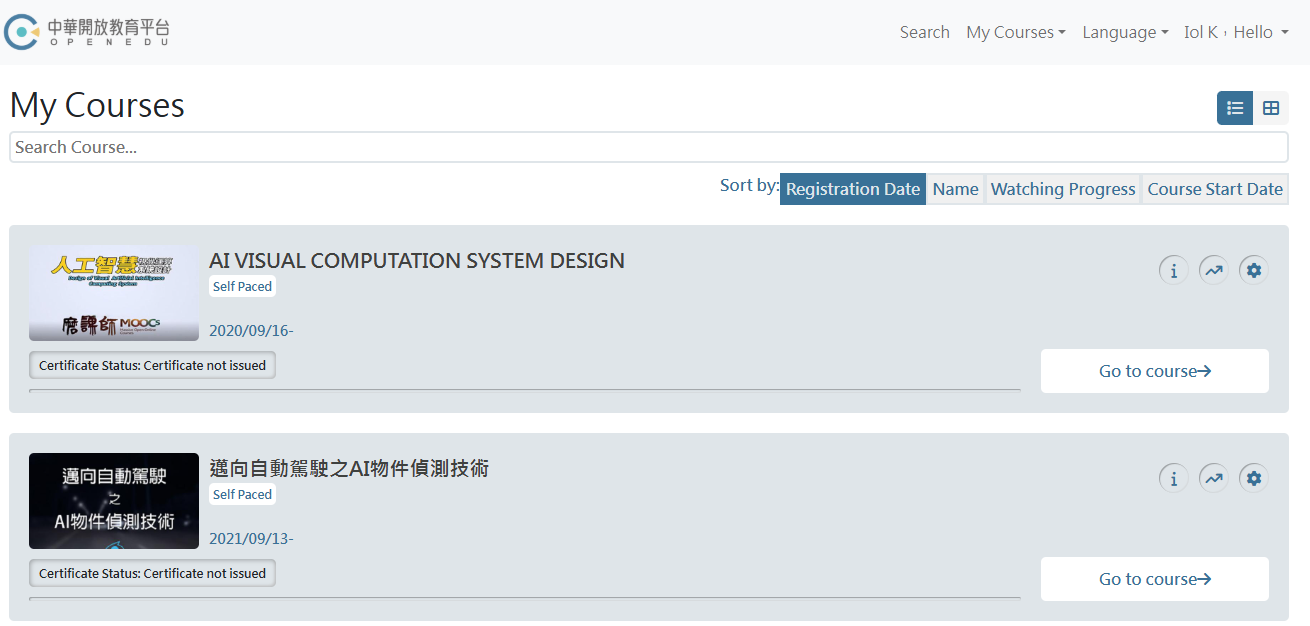
\includegraphics[width=1\textwidth]{./assets/sc1.png}
    \caption{視窗截圖}
    \label{fig:example}
\end{figure}

\newpage

\section{平台使用心得}
\quad\quad
首先,使用上我第一個注意到的事情是影片時間長度,兩個課程都將課程拆成很多部八至二十分鐘的影片,可以依照自身時間彈性調整學習進度,減少了學習的阻力。還有交大課程每個影片後會有一些題目幫助確認是否有吸收,問題的設計是不會有扣分等機制的,在作答上比較沒壓力。另外兩門課主要都是講中文,只有一些專有名詞會用英文,這也減小了學習的阻力。
\begin{figure}[h]
    \centering
    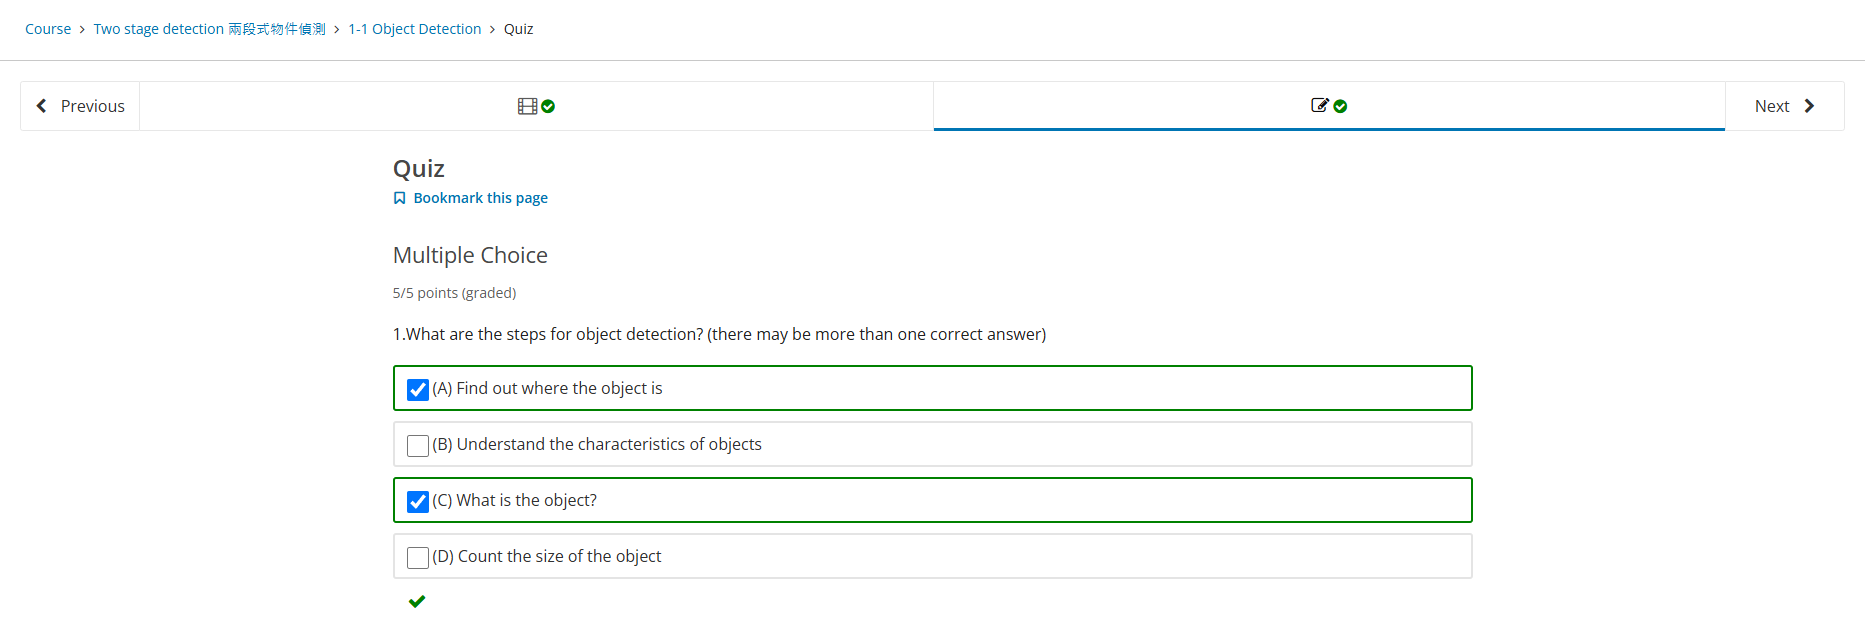
\includegraphics[width=1\textwidth]{./assets/sc3.png}
    \caption{問題題目截圖}
    \label{fig:example}
\end{figure}

再者,交大課程的講解很清楚,影片的圖例顯示與講解方式讓我想到一些國外的youtuber,如\href{https://www.youtube.com/@PolylogCS}{Polylog}、\href{https://www.youtube.com/@PrimerBlobs}{Primer}、\href{https://www.youtube.com/@3blue1brown}{3Blue1Brown}等人,不過他們也有製作動畫等幫助理解。交大的比較像是meeting時報告的樣子,邊說明時旁邊有圖例和專有名詞對理解真的很有幫助,可以較清楚他現在在說什麼。
\begin{figure}[h]
    \centering
    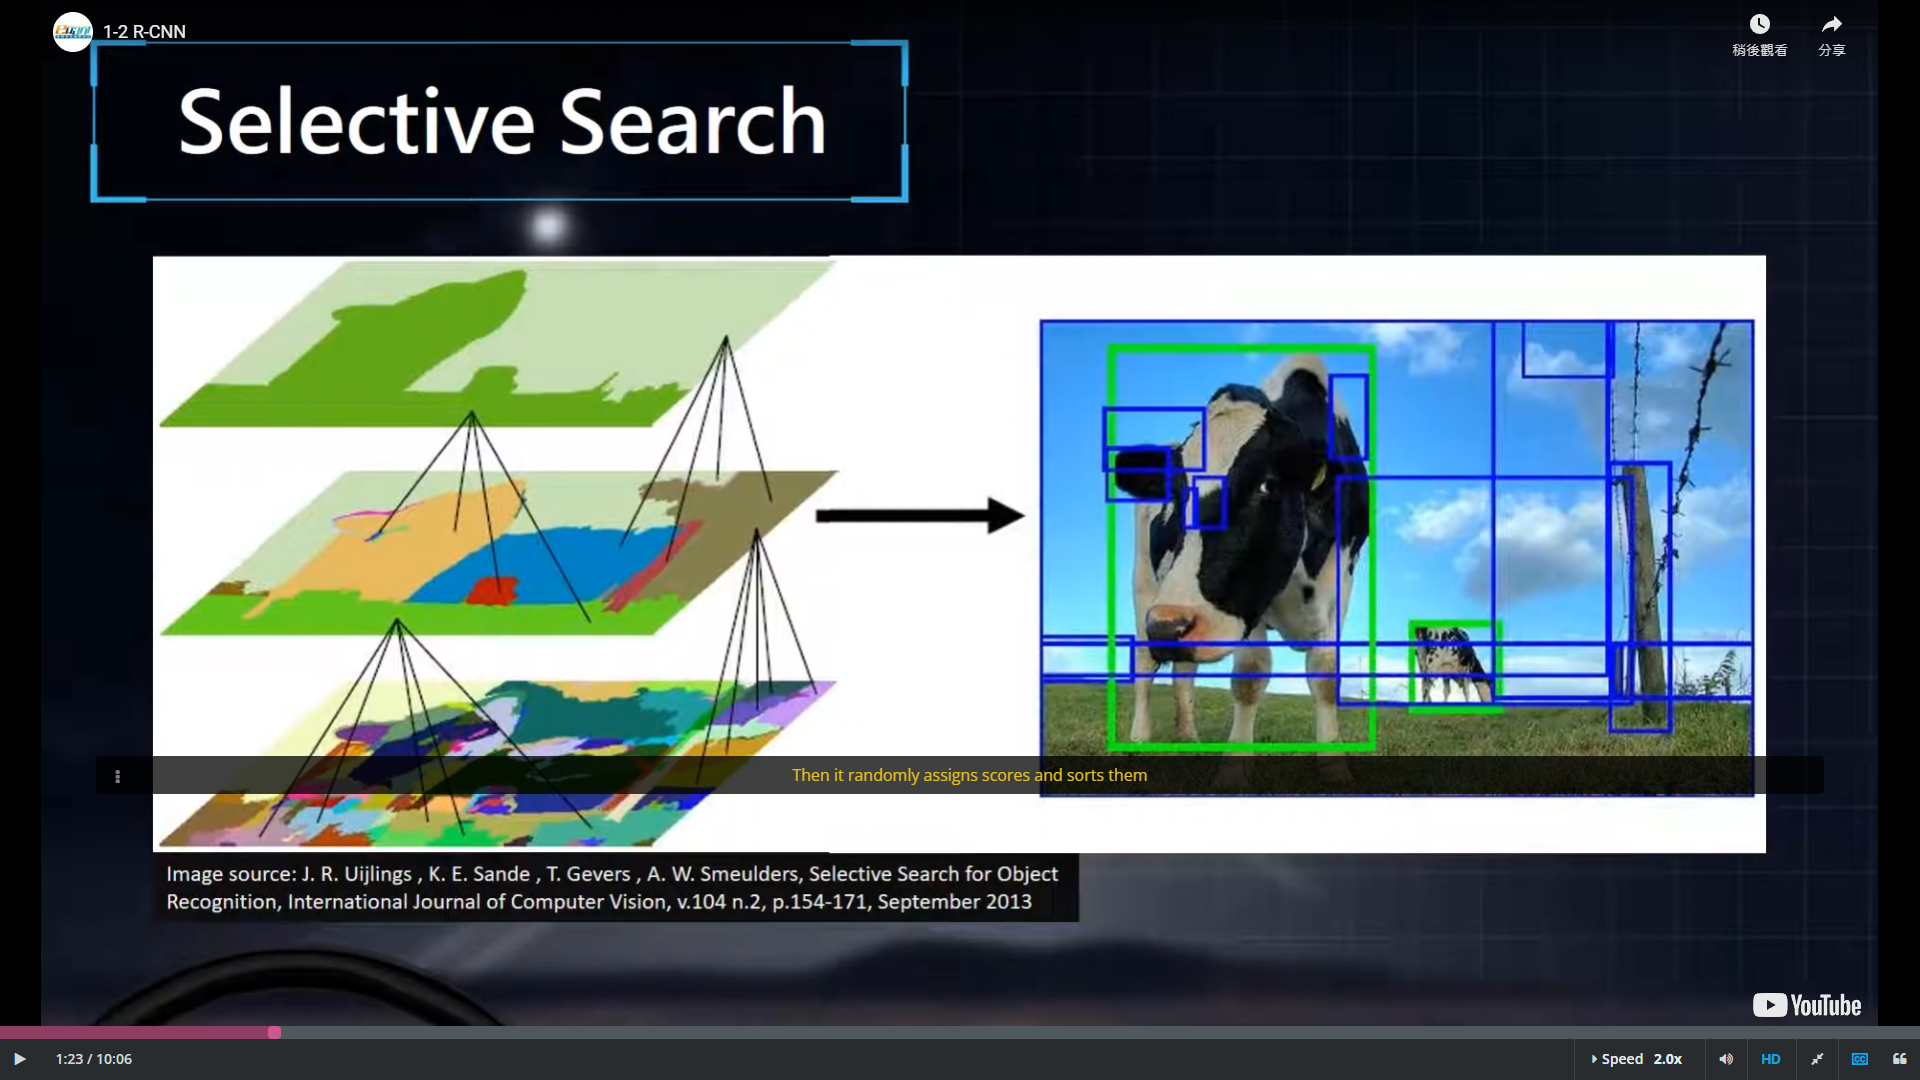
\includegraphics[width=1\textwidth]{./assets/sc2.png}
    \caption{影片截圖}
    \label{fig:example}
\end{figure}

最後說一下目前我認定這兩門課的定位,由於每部影片時間長度不長,內容是精簡的理論與說明,不會有實作教學,但之後自主研究時會比較有方向。另外針對背景知識量不同的學生,收穫跟學習速度會有差異,有些內容會被預設學生已知。


\end{document}